\documentclass[a4paper]{article}

% --- Packages ---

\usepackage{a4wide}
\usepackage[utf8]{inputenc}
\usepackage{amsmath}
\usepackage{mathtools}
\usepackage{amssymb}
\usepackage[english]{babel}
\usepackage{mdframed}
\usepackage{systeme,}
\usepackage{lipsum}
\usepackage{relsize}
\usepackage{caption}
\usepackage{tikz}
\usepackage{tikz-3dplot}
\usetikzlibrary{shapes.geometric}
\usepackage{pgfplots}
\usepackage{pgfplotstable}
\pgfplotsset{compat=newest}%1.7}
\usepackage{harpoon}%
\usepackage{graphicx}
\usepackage{wrapfig}
\usepackage{subcaption}
\usepackage{authblk}
\usepackage{float}
\usepackage{listings}
\usepackage{xcolor}
\usepackage{chngcntr}
\usepackage{amsthm}
\usepackage{comment}
\usepackage{commath}
\usepackage{hyperref}%Might remove, adds link to each reference
\usepackage{url}
\usepackage{calligra}
\usepackage{pgf}

% --- Bibtex ---

%\usepackage[backend = biblar,]{bibtex}

%\addbibliografy(ref.bib)

% --- Commands --- 

\newcommand{\w}{\omega}
\newcommand{\trace}{\text{Tr}}
\newcommand{\grad}{\mathbf{\nabla}}
%\newcommand{\crr}{\mathfrak{r}}
\newcommand{\laplace}{\nabla^2}
\newcommand{\newparagraph}{\vspace{.5cm}\noindent}

% --- Math character commands ---

\newcommand{\curl}[1]{\mathbf{\nabla}\times \mathbf{#1}}
\newcommand{\dive}[1]{\mathbf{\nabla}\cdot \mathbf{#1}}
\newcommand{\res}[2]{\text{Res}(#1,#2)}
\newcommand{\fpartial}[2]{\frac{\partial #1}{\partial #2}}
\newcommand{\rot}[3]{\begin{vmatrix}\hat{x}&\hat{y}&\hat{z}\\\partial_x&\partial_y&\partial_z\\#1&#2&#3 \end{vmatrix}}
\newcommand{\average}[1]{\langle #1 \rangle}
\newcommand{\ket}[1]{|#1\rangle}
\newcommand{\bra}[1]{\langle #1|}


%  --- Special character commands ---

\DeclareMathAlphabet{\mathcalligra}{T1}{calligra}{m}{n}
\DeclareFontShape{T1}{calligra}{m}{n}{<->s*[2.2]callig15}{}
\newcommand{\crr}{\mathcalligra{r}\,}
\newcommand{\boldscriptr}{\pmb{\mathcalligra{r}}\,}


\title{test}
\author{Author : Andreas Evensen}
\date{Date: \today}

% --- Code ---

\definecolor{codegreen}{rgb}{0,0.6,0}
\definecolor{codegray}{rgb}{0.5,0.5,0.5}
\definecolor{codepurple}{rgb}{0.58,0,0.82}
\definecolor{backcolour}{rgb}{0.95,0.95,0.92}

\lstdefinestyle{mystyle}{
    backgroundcolor=\color{backcolour},   
    commentstyle=\color{codegreen},
    keywordstyle=\color{magenta},
    numberstyle=\tiny\color{codegray},
    stringstyle=\color{codepurple},
    basicstyle=\ttfamily\footnotesize,
    breakatwhitespace=false,         
    breaklines=true,                 
    captionpos=b,                    
    keepspaces=true,                 
    numbers=left,                    
    numbersep=5pt,                  
    showspaces=false,                
    showstringspaces=false,
    showtabs=false,                  
    tabsize=2
}

\lstset{style=mystyle}

\begin{document}

%\maketitle

\thispagestyle{empty}
\begin{titlepage}
   \begin{center}
       % \vspace*{1cm}
       \huge
       \textbf{Molecular dynamics: Argon Fluid}\\
       \vspace*{1cm}
       \textbf{Course: FK8028}
       \large

       \vspace*{0.5cm}
       \textbf{Author: Andreas Evensen}\\
       \vspace*{.5cm}
       \small
       \vspace*{1.cm}
       \textbf{Submission date: \today}\\
       \vspace*{.5cm}
       \vspace{0.8cm}
     
       \small
       Stockholm University\\
       Computational Physics\\
       Sweden\\
   \end{center}
\end{titlepage}
\pagenumbering{Roman}
\newpage
\pagenumbering{roman}
\setcounter{page}{1}
\newpage
\tableofcontents
\newpage
\pagenumbering{arabic}

\section{Introduction}
In this report, one simulated an argon fluid, where the atoms interacted with each other through a Lennard-Jones potential.
One evolved the system using a symplectic algorithm, Velocity Verlet, and one analyzed the radial distribution function, the energy in the system as well as the temperature.
Periodic boundary conditions (PBC) were implemented to simulate an infinite system, and the system was evolved in the NVE ensemble, where the number of atoms, the volume, and the energy were conserved; we prove that the energy of the system is conserved.

\newparagraph
The radial distribution function was used to analyze the structure of the fluid, while the energy and temperature were used to analyze the thermodynamic properties of the fluid.
The results showed that the fluid was in a stable state, and that the total energy was conserved in time, whilst the temperature oscillated.
The radial distribution function showed that the fluid was in a liquid state, and that the atoms were distributed in a way that was consistent with a liquid state.

\section{Theory and Methods}
The Hamiltonian of the system, $\mathcal{H}$ is given by the momenta and the potential energy of the system, and is given by:
\begin{align}
    H(t) &= \sum_i \dot{\mathbf{q}}_i\mathbf{p}_i + V(\{\mathbf{q}_i\}). \label{eq: Hamiltonian}
\end{align}This can be written in terms of the kinetic energy and the potential energy $\mathcal{V}$, if the system is conserved:
\begin{align*}
    \mathcal{H} &= \mathcal{K} + \mathcal{V}.
\end{align*}
The temperature of the system is given by the kinetic energy of the atoms, and thus one can compute the temperature in the following manner:
\begin{align}
    T = \frac{2\mathcal{K}}{3Nk_B},\label{eq: Temperature}
\end{align}where $\mathcal{K}$ is the total kinetic energy of the system, of $N$ atoms, and $k_B$ is the Boltzmann constant.
The specific heat capacity can be derived from this result, where the specific heat capacity is given by:
\begin{align}
    C_v = \left(\frac{3}{2k_b} - \frac{4N\average{K}}{k_b^3\average{T}^2}\right)^{-1}\label{eq: heat capacity}.
\end{align}The specific heat capacity is a measurement of the amount of energy that has to be added to the system to increase the temperature by one unit degree per mole.
The radial distribution function states how neighboring atoms are distributed around a given atom, and is given by:
\begin{align}
    g(r) &= \frac{1}{4\pi r^2}\frac{d\rho}{d\mathbf{r}} \label{eq: radial}.
\end{align}The function $\rho$ here is determining the particle density. The radial distribution function thus allows for computing the expected distances between several atoms, and thus gives an indication of the structure of the fluid.
Atoms in a solid structure, i.e. a lattice, will have distinct peaks at distances of the lattice constant, whilst a fluid will have a smoother distribution with a few distinct peaks. A gas will have a very smooth distribution, with no distinct peaks.

\newpage
\section{Results and Discussion}
The system was simulated with a total of $125$ atoms, confined in a cube of length $K \approx 18.2$~Å. The size of the box cube was determined by the density of the fluid, $\rho = 1.4$~g/cm$^3$, and the number of atoms in the system. 
Simulating the system with a larger amount of particles would require a larger box size, to allow for the restricted density.
The simulation was computed with a time-step $\Delta t = 0.001$~ps, and the system was evolved for a total of $20$~ps, i.e. $20000$ time-steps.

\newparagraph
The energy of the system is conserved after the system has reached equilibrium; the system reaches equilibrium shortly after the velocity scaling has ceased.
This is shown in the figure below, where after approximately $0.23$~ps, the system has reached equilibrium, and the Hamiltonian $\mathcal{H}$ is constant.
\begin{figure}[H]
    \centering
    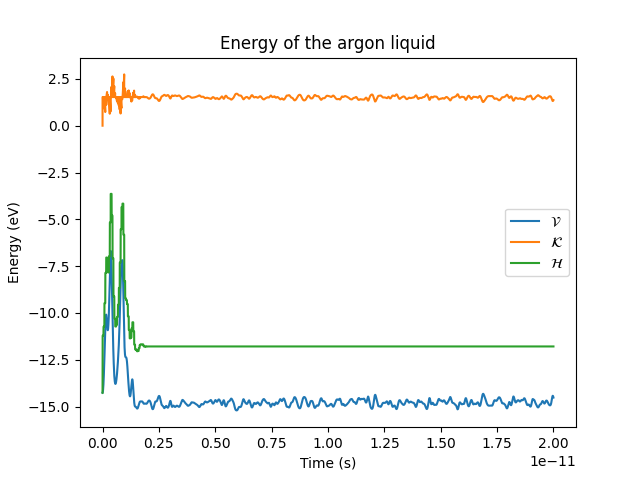
\includegraphics[scale = .5]{energylattice.png}
    \caption{Energy as a function of time}
    \label{fig: energy}
\end{figure}\noindent
The average kinetic energy of the system, after reaching $\average{\mathcal{K}} \approx 1.51$~eV. The average potential energy is $\average{\mathcal{V}} \approx -14.79$~eV.
This can also be visualized in the figure above, fig \ref{fig: energy}, where it's seen that the kinetic energy is oscillating around the given value, as well as the potential energy.

\newparagraph
The temperature of the system, after the rescaling has ceased, is fluctuating around the fixed temperature of $94.4$~K, as shown in the figure below, fig \ref{fig: temperature}.
The average temperature of the system, after reaching equilibrium, is $93.1$~K. This number varies slightly from the fixed temperature, which is due to the number of times the rescaling has occurred; increasing this number will decrease the difference between the fixed temperature and the average temperature.
\begin{figure}[H]
    \centering
    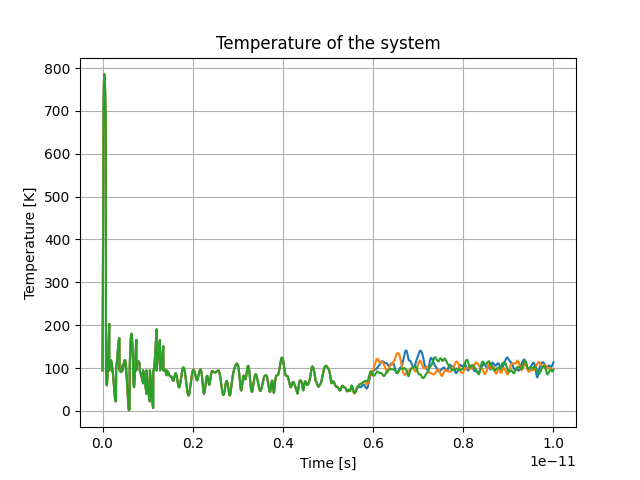
\includegraphics[scale = .5]{temperature.png}
    \caption{Temperature distribution in the liquid.}
    \label{fig: temperature}
\end{figure}\noindent
The radial distribution function, eq \eqref{eq: radial}, is computed for the system after it has reached equilibrium, and is shown in the figure below, fig \ref{fig: radial}.
It's computed for a variety of instances in time, to visualize the change in the radial distribution, as a function of time.
\begin{figure}[H]
    \centering
    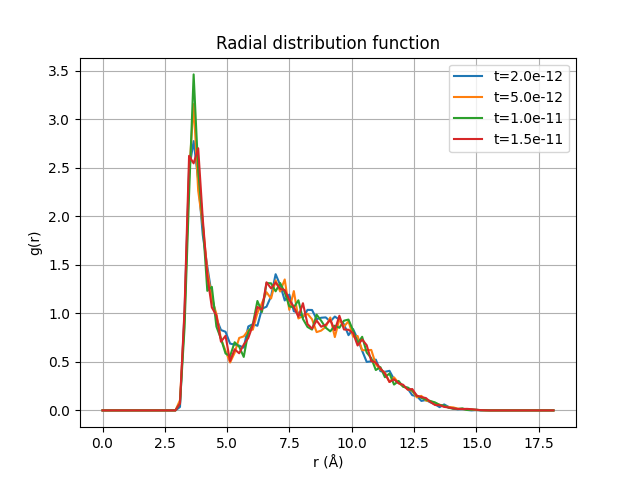
\includegraphics[scale = .5]{radial.png}
    \caption{Radial distribution of the state.}
    \label{fig: radial}
\end{figure}\noindent
The radial distribution function, after the system has reached equilibrium, is computed over the average of each iteration, and thus this visualizes the distance between the atoms. This is shown in figure \ref{fig: average radial}.
One sees that the first peak is around $3.75$~Å, which is consistent with the Lennard-Jones potential, which has a minimum at $3.8$~Å, for Argon interactions.
The second peak is around $7.3$~Å, which means that the distance between the second neighbor is around $7.3$~Å, in other words, that there exist an atom at a distance $3.75$~Å in between the two atoms.

\newparagraph
The last peak is located around $8.7$~Å, which means that the third neighbor is located at a distance of $8.7$~Å, from the atom.
This is in contrary to the value given by Rahman[2]; he found that the third peak was located at $10.4$~Å, which is a significant difference. The reason for this is due to our box size when computing with the periodic boundary condition.
The box-size is approximately $18.2$~Å, and the atoms are distributed in a way such that the third peak is located approximately at half of the box size width. The shape of the average radial distribution, fig \ref{fig: average radial} is consistent with that of a liquid.

\newparagraph
The radial distribution function, before the system has reached equilibrium, is shown in figure \ref{fig: before radial }.

\begin{figure}[H]
    \centering
    \begin{subfigure}[b]{0.45\textwidth}
        \centering
        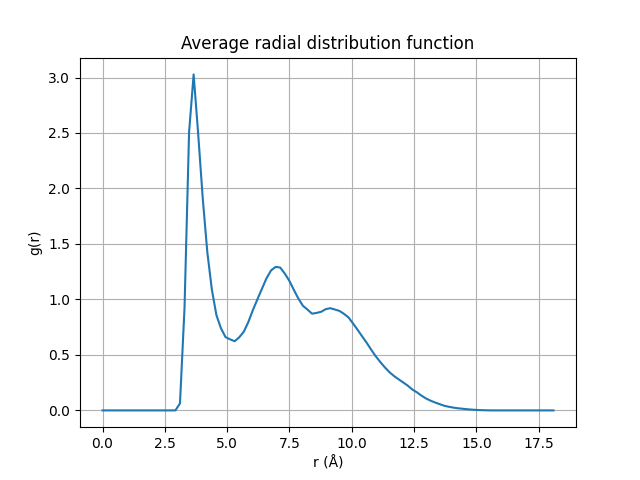
\includegraphics[width=\textwidth]{average_radial.png}
        \caption{Average radial distribution function after equilibrium.}
        \label{fig: average radial}
    \end{subfigure}
    \hfill
    \begin{subfigure}[b]{0.45\textwidth}
        \centering
        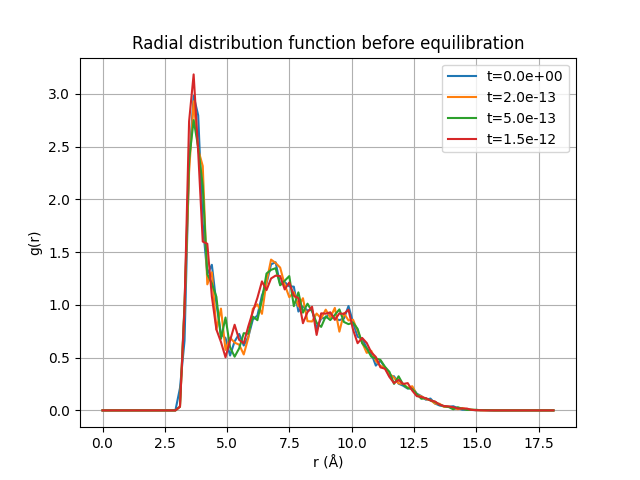
\includegraphics[width=\textwidth]{radial_before.png}
        \caption{Radial distribution function before equilibrium.}
        \label{fig: before radial }
    \end{subfigure}
    \caption{(a) Shows the average radial distribution function after the system has reached equilibrium. (b) shows the radial distribution function before the system has reached equilibrium.}
    \label{fig: Radial tests}
\end{figure}\noindent
The specific heat capacity was computed, according eq \eqref{eq: heat capacity}, to be $C_v = 23.83$~J/(mol K).
This is consistent with the specific heat capacity of Argon, which is $C_v = 20.7$~J/(mol K) for a slightly lower temperature, and thus the system is in a stable state, and the specific heat capacity is consistent with the specific heat capacity of Argon[1].


\section{Conclusion}
The system models liquid Argon, at a fixed temperature. The system fluctuate violently in the begging of the simulation due to velocity scaling: to achieve the fixed temperature.
As the system equilibrates, the Hamiltonian of the system becomes constant which is expected. The temperature of the system fluctuates around the fixed temperature, which is expected in the given NVE ensemble.

\newparagraph
The radial distribution function gives an indication of the structure of the fluid, and as the system equilibrates, the radial distribution function becomes smoother, and the peaks become more pronounced. This shows that the fluid is in a stable state.
Moreover, the radial distribution function is giving information about the distance between neighboring atoms, and the peaks are consistent with that of the Lennard-Jones potential which is used to model the interactions between the atoms.

\newparagraph
The simulation was written in a compiled language (V) which is a statically typed language. The features of the languages allowed for a fast and efficient simulation, and the results were consistent with the expected results. 
The simulation could be improved by parallelizing the code, and using so-called "cut-offs" to reduce the number of interactions that are computed.


\newpage
\section{Reference}
[1] NIST (2024), \url{https://webbook.nist.gov/cgi/cbook.cgi?ID=C7440371&Mask=1&Type=JANAFG&Table=on}\newline
[2] A. Rahman (1964) Correlation in the Motion of atoms in liquid Argon, Phys. Rev. 136, A405-A411
\end{document}
 
